\chapter{Implementation}\label{sec:implementation}

This section describes the reference implementation for the conceptual framework in Chapter \ref{cha:concept}.
Various components and interaction techniques of the geographical visualization are detailed.
The integration of the geographical visualization in the existing \visan{} is shown.
The connection of the conceptual framework and the implemented framework is examined.

\section{Geographical visualization with React and Leaflet}

The geographical visualization is implemented as a \attr{Map} component of the React Leaflet library.
Listing \ref{lst:implementation:render} shows the \attr{render} method of the component.

\lstinputlisting[
  language=JavaScript,
  label={lst:implementation:render},
  caption={\attr{render} method of the Map component of the geographical visualization}
]{listings/implementation/render.tsx}

The \attr{render} method is the only required method of a React component.
It will be invoked on the initial rendering of the component of the \attr{DOM} and on every update of the component's properties.
React's templating language ``\attr{JSX}'' allows to nest other child components in to the React parent component.
In this case the \attr{Map} component includes a \attr{TileLayer} \attr{GeoJSON} component from the \attr{react-leaflet} library.
This library conveniently provides ``React components for Leaflet maps.''~\cite{ReactLeaflet2017}.

\subsection{GeoJSON component}

The \attr{GeoJSON} component is provided by the \attr{Map} component with a couple of properties:
It gets a
\begin{enumerate*}[label=(\arabic*)]
  \item
    geojsonURL as well as a
  \item
    geojson as data attribute. Furthermore a couple of callbacks is passed into the child component, including
  \item
    featureStyle,
  \item
    pointToLayer and
  \item
    onEachFeature.
\end{enumerate*}

This way, the parent \attr{Map} component controls the data flow and without a \attr{geojson} object, no polygons are placed on the map.
A changed \attr{geojsonURL} will always update the child component as it is used a \attr{key} on the \attr{GeoJSON} component.
The callbacks passed into the \attr{GeoJSON} component control the visual representation of each polygon and they add event handlers for a mouse click or a mouse move on each polygon.
Listing \ref{lst:implementation:onEachFeature} shows the event handlers added to the map.

\lstinputlisting[
  language=JavaScript,
  label={lst:implementation:onEachFeature},
  caption={\attr{onEachFeature} callback passed into the \attr{GeoJSON} component, adding handlers for mouse events}
]{listings/implementation/onEachFeature.tsx}

First we cache all layers in the internal state of the \attr{Map} component.
On each \attr{mouseover} event, the \attr{id} of the feature is published as \attr{mcv.select.highlight} interaction.
A \attr{click} event is distinguised if the control key is pressed or not.
In the latter case, the id of the feature is either added or removed from the list of focused ids and then the list of focused ids is published as \attr{mcv.select.focus} interaction.

\lstinputlisting[
  language=JavaScript,
  label={lst:implementation:featureStyle},
  caption={\attr{featureStyle} callback passed into the \attr{GeoJSON} component, configuring the visual appearance depending on the currently highlighted or focused feature ids}
]{listings/implementation/featureStyle.tsx}

The \attr{featureStyle} method is very straightforward.
If the feature is currently focused, the \attr{fillColor} of the polygon is red, otherwise blue.
Likewise, if the feature is currently highlighted, the polygon has a white, solid stroke.







\section{Implemented interactions}

In the course of this thesis we want to implement the following interactions:
\begin{itemize}
  \item
    \emph{Select}: The user clicks on a building or region in a geographical map and all affected properties in the \tmap{} will be highlighted.
  \item
    \emph{Explore}: The user clicks on a block in the \tmap{} and the viewpoint in the geographical map will be centered on relevant area.
  \item
    \emph{Reconfigure}: The user selects a different feature set and the changes are reflected in both the geographical map (e.g. point instead of polygon geometries) and in the \tmap{}.
  \item
    \emph{Filter}: The user double-clicks on a region in a geographical map and the \tmap{} will be based on data of only that region.
\end{itemize}

\section{Standards}
\todo[inline]{no section without text}

\textbf{GeoJSON} is the name of the data format used to exchange geometries.

An example of aggregated user data merged with geometry data can be seen in listing~\ref{lst:geojson:example}.
\lstinputlisting[language=JavaScript, label={lst:geojson:example}, caption={Geojson example}]{listings/example.geojson}

We can use this data as input for our common \visan{}, e.g.\ figure~\ref{fig:implementation:user_distribution} shows the user distribution of \rufu{}.

\begin{figure}[h!]
  \centering
  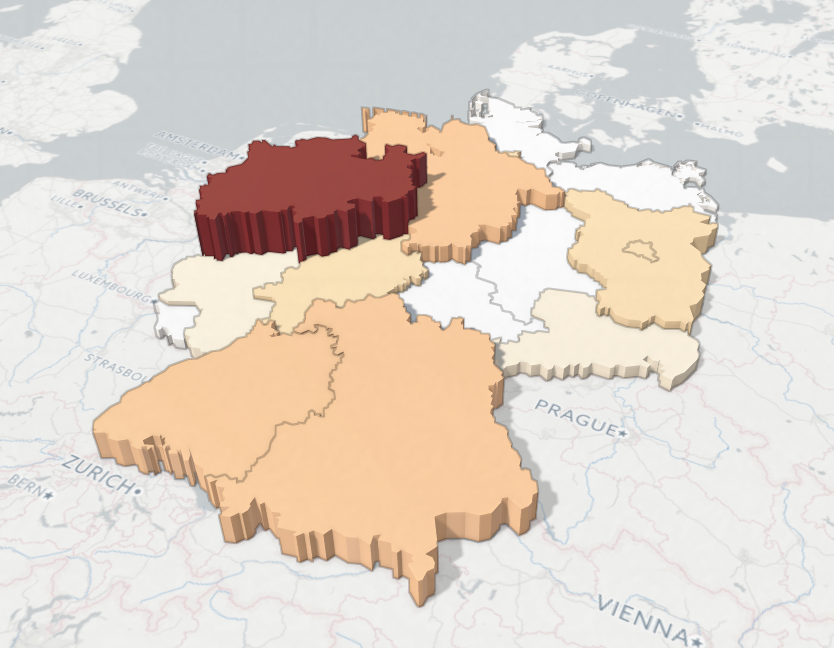
\includegraphics[width=\textwidth]{images/ua_example.png}
  \caption{%
    User distribution of \rufu{} across German federal states
  }\label{fig:implementation:user_distribution}
\end{figure}

\textbf{Web components} is a recent standard of the W3C\cite{W3C2017} to bring component-based software engineering to the world wide web.
They look perfectly suited to be used in \cmvs{}.
However the attributes of web components are string based.
If arbitrary javascript objects need to be passed into the web component it is suggested to use one of the common javascript frameworks that allow for data binding.

\section{Software patterns}
Figure~\ref{fig:implementation:sequence-diagram} shows how \cmvs{} can be automatically updated even if the environment lacks a native update-mechanism.

\begin{figure}[h!]
  \centering
  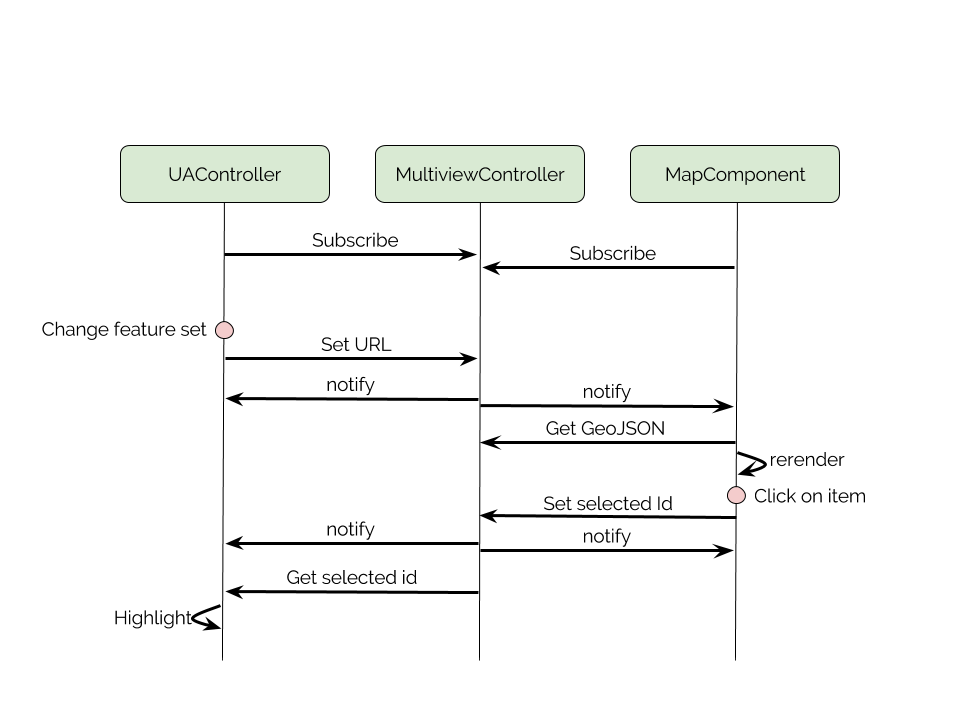
\includegraphics[width=\textwidth]{images/sequence-diagram.png}
  \caption{%
    The sequence diagram shows the notification of different components.
  The user first chooses a feature set and hovers over a polygon in the geographical map.
  }\label{fig:implementation:sequence-diagram}
\end{figure}


\textbf{The Observer pattern} allows multiple \emph{observers} to react to changes of an observed state.
In our case, the observed state is the \attr{MultiviewController}.
Any change to the \attr{MultiviewController} will subsequently be broadcasted to all connected views.


\textbf{Publisher subscriber}
In our particular case we apply a special form of the observer pattern, the so called ``Publish-subscribe'' pattern\cite{Eugster2003}.
Publish-subsribe is a messaging pattern which is widely used in message queues.
In this scenario, senders of messages simply categorize their messages which will be consumed by subscribers of the category.
The scenario has very low coupling, publishers do not even need to know the existence of subscribers.

\textbf{Component pattern}
State-of-the-art javascript component frameworks like ReactJS and EmberJS follow the component pattern for the architecture of a single page web application.
The component pattern imposes a hierarchical structure on a website.
Each component is responsible for a task and may contain other components.
The components are joined at the root node of the page.

This pattern is very applicable to \cmvs{}.
The different views of \cmvs{} share state, i.e.\ the feature, that is currently highlighted or the applied filter on the data.
So the views are components and their closest common ancestor is the \cmv{} itself, controlling state and passing user interaction down to it's children.

\begin{figure}[h!]
  \centering
  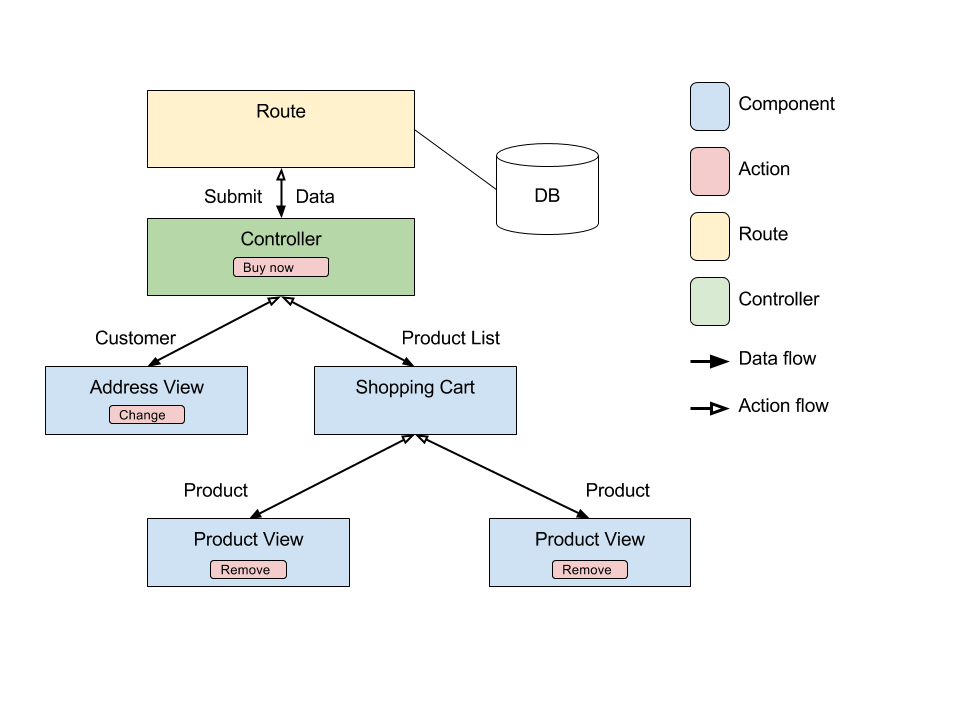
\includegraphics[width=\textwidth]{images/data-down-actions-up.png}
  \caption{%
    Implementation of the component pattern in EmberJS\@.
    The example shows a page of a webshop.
    The customer is about to order the items in the shopping cart.
  }\label{fig:implementation:data-down-actions-up}
\end{figure}

\textbf{Actions up --- Data down}

Version 2.0 of Ember introduced a common phrase how to use this pattern effectively: ``Data down, actions up''\cite{Emberigniter2017}
In the domain of \cmvs{} actions would mean user interactions, e.g.\ a click on a feature.
The action will notify the controlling \cmv{} component.
Actions may change data, and the changes will be passed to to all dependen views.
These views are then rerendered.

Examples for the kind of data that might trigger a rerendering of a view:
\begin{itemize}
  \item
    The selected feature or a list of selected features
  \item
    A list of thresholds for certain features as a filter
\end{itemize}
\section{Geographical Data Visualization}

\todo[inline]{Introduce the implementation of the geographical map}


\subsection{Client-side component frameworks}

We evaluated three javascript component frameworks for our application: \emph{GlimmerJS}, \emph{Google Polymer} and \emph{ReactJS}.
Figure~\ref{fig:implementation:frontend-frameworks} shows the pros and cons of each framework for our use case.

\textbf{GlimmerJS} is the rendering enginge of EmberJS\cite{Ember2017}.
In 2017 it was released as a standalone component framework.
Applications written in GlimmerJS can be exported as web components.
These web components can be included in any website, which makes GlimmerJS a reasonable choice to build high-quality widgets for user interfaces.
GlimmerJS also uses handlebars\cite{Handlebars2017}, a user-friendly templating language.
The downside of GlimmerJS is the current lack of documentation and immaturity due to the recent first release this year.

\textbf{Google Polymer} is another popular library to build web components \cite{Polymer2017}.
With 18,469 stars on Github it is the most popular framework for web components at the time of writing.
Polymer has a large community and comprehensive documentation and therefore more suitable than GlimmerJS for our task.

Unfortunately, the web component standard does not specify how arbitrary Javascript objects can be passed to web components.
This raises some problems in legacy apps:
Usually, legacy apps are written in plain javascript without the use of a component-based frontend framework.
Any part of the code may call any other part of the code, leading to the dreaded ``spaghetti code''.
Refactoring the existing app requires the framework to have a reliable way of communication with the legacy parts.
E.g.\ parts of the legacy code call the backend in order to load data.
This data needs to be passed to the components of the user interface.
Web components do not have a designated interface
Because of that, libraries like Polymer come back on proprietary solutions.
But those proprietary solutions defeat the main advantage of developing against a standard, as it is unclear how components may interact with each other.

\textbf{ReactJS} is a JavaScript library for building user interfaces\cite{React2017}.
After lifting the constraint to implement against web components, it is the javascript framework we finally decided to go for.
ReactJS does not have the ability to export web components.
It has, in return, an ascertained way of integrating the component framework into a legacy app built with jQuery.
Along with its major advantage of easy integration, it has a striving community, heaps of documentation and tutorials and is well tested.

All of these reasons make us choose ReactJS for the task of coordinating multiple views in our existing \visan{}.


\todo[inline]{Pros/cons of GlimmerJS, Polymer, React}


\begin{figure}[h!]
  \centering
  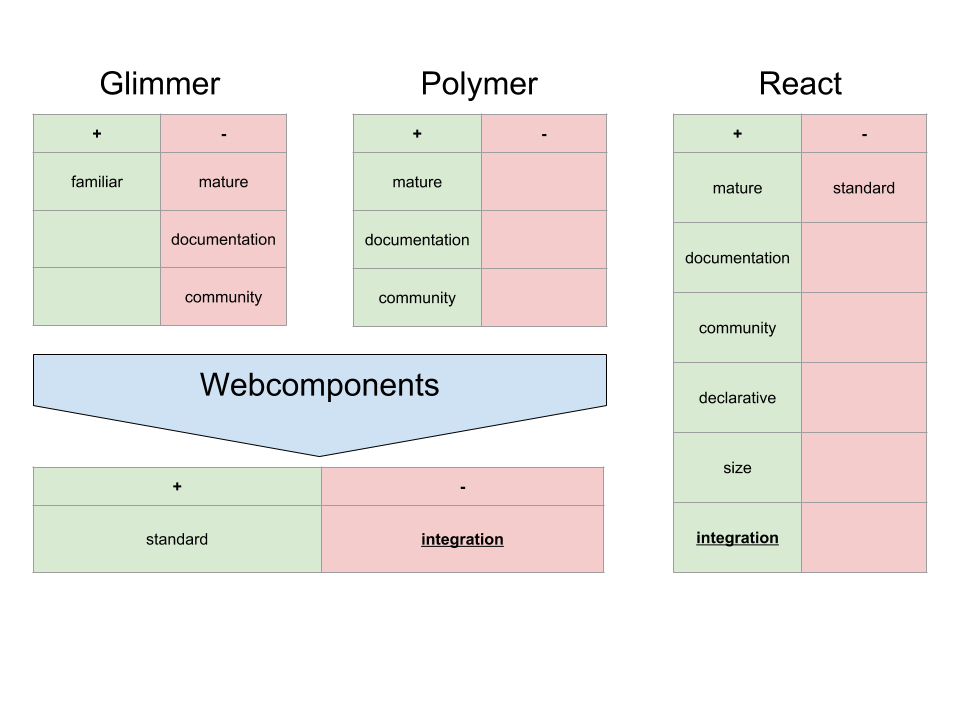
\includegraphics[width=\textwidth]{images/frontend-frameworks.png}
  \caption{Comparison of frontend frameworks}\label{fig:implementation:frontend-frameworks}
\end{figure}


\begin{figure}[h!]
  \centering
  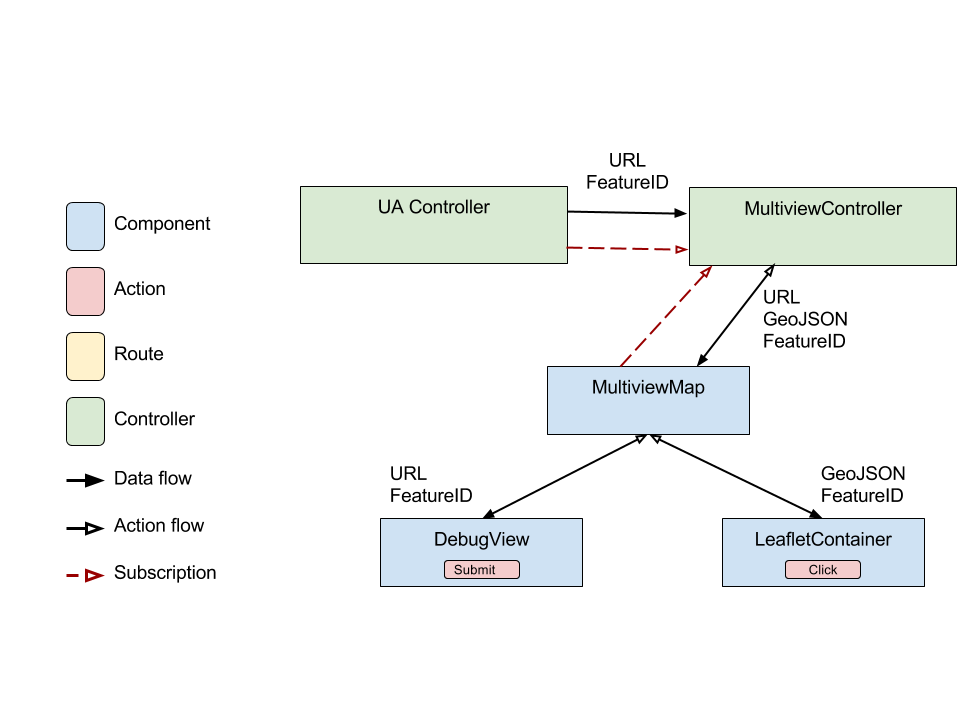
\includegraphics[width=\textwidth]{images/both-patterns-implemented.png}
  \caption{%
    Both observer pattern and component pattern applied in the field of \cmvs{}
  }\label{fig:implementation:both-patterns}
\end{figure}


\textbf{Leaflet}
Leaflet is the leading open-source JavaScript library for mobile-friendly interactive maps~\cite{Leaflet2017}.
\todo[inline]{Show a code example how to use Leaflet}

\textbf{PubSubJS}
PubSubJS is a topic-based publish/subscribe library written in JavaScript~\cite{PubSubJS2017}.
Topics are published asynchronuously.
\todo[inline]{Show a code listing here, how interaction verbs are mapped to topics}

\section{Coordination of Geographical Visualization and Treemap}

\todo[inline]{Introduce how we integrated the geographical map into the existing
treemap implementation}

\textbf{Observer pattern and component pattern in \cmvs{}}
Figure~\ref{fig:implementation:both-patterns} shows the final result.
We try to put as much code as possible under the root node of ReactJS\@.
By that we eliminate the amount of custom updating implementation.
The root node of the DOM-tree of our react application is connected with the existing app through the common interface.
Both urban analytics controller and the multiview map component will observe changes to the common interface.
Also sub-components may communicate with the common interface.
